\documentclass[12pt, compress]{beamer}

\usetheme[numbering=fraction, progressbar=none, titleformat=smallcaps, sectionpage=none]{metropolis}

\usepackage{sourcecodepro}
\usepackage{booktabs}
\usepackage{array}
\usepackage{listings}
\usepackage{graphicx}
\usepackage[english]{babel}
\usepackage[scale=2]{ccicons}
\usepackage{url}
\usepackage{relsize}
\usepackage{wasysym}

\usepackage{pgfplots}
\usepgfplotslibrary{dateplot}

\definecolor{Base}{HTML}{191F26}
\definecolor{Accent}{HTML}{157FFF}

\setbeamercolor{alerted text}{fg=Accent}
\setbeamercolor{frametitle}{bg=Base}

\setsansfont[BoldFont={Source Sans Pro Semibold},
              Numbers={OldStyle}]{Source Sans Pro}

\lstset{ %
  backgroundcolor={},
  basicstyle=\ttfamily\footnotesize,
  breakatwhitespace=true,
  breaklines=true,
  captionpos=n,
  commentstyle=\color{Accent},
  escapeinside={\%*}{*)},
  extendedchars=true,
  frame=n,
  keywordstyle=\color{Accent},
  language=C++,
  rulecolor=\color{black},
  showspaces=false,
  showstringspaces=false,
  showtabs=false,
  stepnumber=2,
  stringstyle=\color{gray},
  tabsize=2,
  keywords={thrust,plus,device_vector, copy,transform,begin,end, copyin,
  copyout, acc, \_\_global\_\_, void, int, float, main, threadIdx, blockIdx,
  blockDim, if, else, malloc, NULL, cudaMalloc, cudaMemcpy, cudaSuccess,
  cudaGetLastError, cudaDeviceSynchronize, cudaFree, cudaMemcpyDeviceToHost,
  cudaMemcpyHostToDevice, const, data, independent, kernels, loop,
  fprintf, stderr, cudaGetErrorString, EXIT_FAILURE, for, dim3},
  otherkeywords={::, \#pragma, \#include, <<<,>>>, \&, \*, +, -, /, [, ], >, <}
}

\renewcommand*{\UrlFont}{\ttfamily\smaller\relax}

\graphicspath{{../img/}}

\title{Introdução a Message Passing Interface (MPI)}
\author{\footnotesize Pedro Bruel \\ {\scriptsize \emph{phrb@ime.usp.br}}}
\institute{
\includegraphics[height=2cm]{imelogo}\\[0.2cm] Instituto de Matemática e Estatística \\ Universidade de São Paulo}
\date{\scriptsize \today}

\begin{document}

\maketitle

\section{Introdução}

\begin{frame}
    \frametitle{Slides}
    \begin{center}
        
\includegraphics[width=.18\textwidth]{github}
    \end{center}
    Os slides e todo o código fonte estão no \alert{GitHub}:

    \begin{itemize}
        \item \url{github.com/phrb/aula-mpi}
    \end{itemize}
\end{frame}

\begin{frame}
    \frametitle{Modelos de Programação Paralela}
    \begin{itemize}
        \item Interação entre processos:
            \begin{itemize}
                \item Memória compartilhada: pthreads, OpenMP
                \item \alert{Troca de mensagens}: Message Passing Interface (MPI)
                \item Interação implícita: Paralelização automática
            \end{itemize}
    \end{itemize}

    \begin{itemize}
        \item Decomposição do problema:
            \begin{itemize}
                \item \alert{Paralelismo de tarefas}: MPI
                \item Paralelismo de dados: GPUs
                \item Paralelismo implícito: \textit{instruction-level parallelism}
            \end{itemize}
    \end{itemize}
\end{frame}

\begin{frame}
    \frametitle{Message Passing Interface (MPI)}
    \begin{center}
        
\includegraphics[width=.3\textwidth]{mpi-logo}
    \end{center}

    Message Passing Interface (\alert{MPI}):

    \begin{itemize}
        \item \alert{Troca de mensagens} entre \alert{processos}
        \item \alert{Padronizado} e \alert{portável}
        \item Implementações em diversas \alert{linguagens} e
            \alert{arquiteturas}
    \end{itemize}
\end{frame}

\begin{frame}
    \frametitle{MPI: Conceitos Básicos}
    \begin{center}
        
\includegraphics[width=.3\textwidth]{mpi-logo}
    \end{center}

    Conceitos básicos:

    \begin{itemize}
        \item \alert{Communicator}
        \item \alert{Point-to-Point} communication
        \item \alert{Collective} communication
        \item \alert{Datatypes}
    \end{itemize}
\end{frame}

\begin{frame}
    \frametitle{MPI: Modelo de Programação}
    \begin{center}
        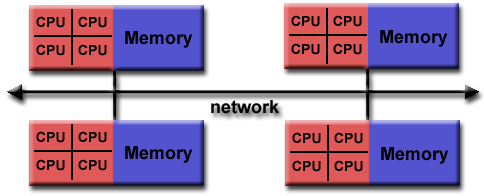
\includegraphics[width=\textwidth]{hybrid-mem}
    \end{center}
\end{frame}

\begin{frame}
    \frametitle{Usando MPI + OpenMP}
    \begin{center}
        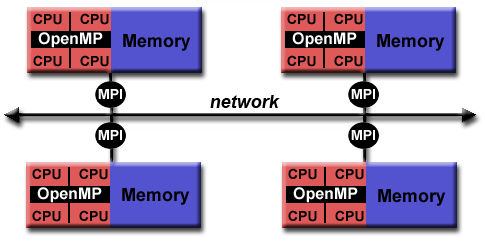
\includegraphics[width=\textwidth]{hybrid-model}
    \end{center}
\end{frame}


\begin{frame}
    \frametitle{OpenMPI}
    \begin{center}
        
\includegraphics[width=.3\textwidth]{open-mpi-logo}
    \end{center}

    \alert{OpenMPI}:

    \begin{itemize}
        \item Implementação \alert{open-source} do padrão MPI
        \item Bastante usado em supercomputadores da \alert{TOP 500}
        \item \url{open-mpi.org}
        \item \url{github.com/open-mpi/ompi}
    \end{itemize}
\end{frame}

\begin{frame}
    \frametitle{API e Exemplos}
    \begin{itemize}
        \item \alert{Tutorial}: \url{computing.llnl.gov/tutorials/mpi}
        \item \alert{Código}: \url{github.com/phrb/aula-mpi}
        \item \alert{Documentação}: \url{open-mpi.org/doc/current}
    \end{itemize}

    Vamos usar MPI para:

    \begin{itemize}
        \item Comunicação simples: \textit{blocking} \& \textit{nonblocking}
        \item Calcular $\pi$: \textit{reduce} \& \textit{send}
        \item Calcular números primos
        \item Medir largura de banda da comunicação
        \item Calcular dissipação de calor 2D
    \end{itemize}
\end{frame}

\maketitle

\end{document}
